\documentclass[a4paper]{article}

%% Language and font encodings
\usepackage[english]{babel}
\usepackage[utf8x]{inputenc}
\usepackage[T1]{fontenc}

%% Sets page size and margins
\usepackage[a4paper,top=3cm,bottom=2cm,left=3cm,right=3cm,marginparwidth=1.75cm]{geometry}

%% Useful packages
\usepackage{amsmath}
\usepackage{amssymb}
\usepackage{float}
\usepackage{graphicx}
\usepackage[colorinlistoftodos]{todonotes}
\usepackage[colorlinks=true, allcolors=blue]{hyperref}

\title{Deriving the Ideal Gas Laws}
\author{Jacob Santry}

\begin{document}
\maketitle


\section{Derivation of Kinetic Energy Equation}

\subsection{Change in Momentum}

The change in momentum is equal to the initial momentum. \[ \text{Let}\ P=\text{mu}. \]
as the collision is elastic the speed remains the same but in the opposite direction.
\[ \text{Let}\ \Delta P=\text{-mu-mu}=\text{(-)2mu} \]

\small *This assumes that the collisions are elastic. \normalsize
\subsection{Number of Collisions per Second}

As \[\text{Number of collisions per second} = \frac{1}{\text{time for one collision}}\]
and the time it takes to collide again is equal to the time it takes to travel the distance of the box and back again at its speed
\[ \text{Let} \text{Number of collisions per second} = \frac{1}{\frac{2l}{u}} = \frac{u}{2l} \]

\small *This assumes that the time for the collision is much less than the time between collisions.\normalsize
\subsection{Change in Momentum per second/ Force}

Change in momentum per second is equal to the change in momentum which we have and the number of collisions per second which we also have. Therefore:
 \[\text{Change in Momentum per second} = F = 2mu \times \frac{u}{2l} = \frac{mu^2}{l}\]

\begin{figure}
\centering
\end{figure}

\subsection{Pressure exerted by the particle(s) on the surface}

Pressure equals force over areas the force being the change in momentum divided by the time taken with the area being the surface of the box that the particle will collide with A = \(l^2\).  $\therefore$

\[P = \frac{F}{A} = \frac{mu^2}{l^3}\]

Thus for N particles you get the equation:

\[P = \frac{Nmu^2}{l^3}\]

\[ \text{Let} V=l^3 \]

\[ pl^3 = pV = Nmu^2 \]

\subsection{Root Mean Squared Speed}

\begin{figure}[H]
	\centering
	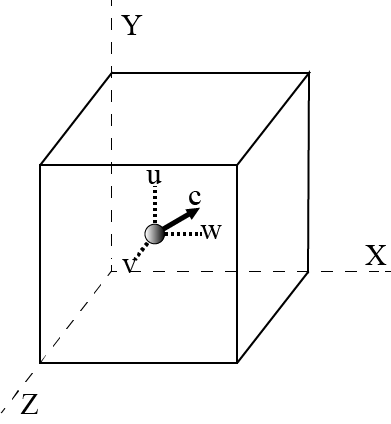
\includegraphics[width=0.35\textwidth]{Diagrams/rootspeed}
	\caption{Velocity components of a gas particle}
\end{figure}

Take any particle its speed c is split into the 3 components of x,y,z this gives:

\[C = \sqrt[]{u^2+v^2+w^2}\]

The mean speed of the particles is then:

\[\overline{c}^2 = \overline{u}^2 + \overline{v}^2 + \overline{w}^2\]

As the average particle speeds in x,y,z should be equivalent, then

\[\overline{u}^2 = \frac{1}{3}\overline{c}^2 \]
\small *This assumes that there are many particles and that they have a random motion and that the volume of the container is much larger than the volume of the particles.\normalsize
\subsection{Putting the derivation together}

So far we have:
\[\Delta P=\text{-mu-mu}=\text{(-)2mu} \]

\[F = 2mu \times \frac{u}{2l} = \frac{mu^2}{l}\]

\[ pV = Nmu^2 \]
and
\[\overline{u}^2 = \frac{1}{3}\overline{c}^2 \]
Substituting in the value for root mean speed into the pressure exerted on the wall be N particles gives us
\[pV = \frac{1}{3}Nm \overline{c}^2\]

Which is the equation for the kinetic energy of a gas. Success!

\end{document}
